\documentclass[fleqn,10pt]{wlscirep}
\usepackage[utf8]{inputenc}
\usepackage[T1]{fontenc}
\usepackage{placeins}

\title{Mechanics-informed crack localization from raw multiplexed fiber Bragg grating signals}

\author[a,c]{A.~Uğurveren}
\author[a]{A.~Gros}
\author[a,c]{E.~Nohutcuoğlu}
\author[a,c]{T.~Tekoğlu}
\author[c]{K.~Yüksel}
\author[a]{K.~Chah}
\author[a,b,*]{C.~Caucheteur}

\affil[a]{Electromagnetism and Telecommunication Department, UMONS, Mons, 7000, Belgium}
\affil[b]{WEL Research Institute, Avenue Pasteur, 6, 1300 Wavre, Belgium}
\affil[c]{FISENS, Izmir Institute of Technology, Urla, 35430, Türkiye}
\affil[*]{christophe.caucheteur@umons.ac.be}

%\keywords{fiber Bragg grating, structural health monitoring, crack localization, deep learning, mechanics-informed learning}

\begin{abstract}
Accurate localization of crack initiation from optical fiber measurements remains a challenge in structural health monitoring. Existing approaches rely on engineered spectral features, or distributed sensing, which can limit direct detection of localized damage from raw signals. Here, we present a mechanics-informed learning framework for crack localization from short temporal windows of raw multiplexed fiber Bragg grating (FBG) interrogator signals. The method combines multichannel temporal inputs with descriptors derived from beam mechanics, including expected elastic strain and deviations between measured and predicted responses. A multiscale temporal convolutional neural network classifies windows associated with cracks, while an auxiliary loss based on mechanics incorporates elastic behavior before crack initiation during training. Experiments on glass fiber composite beams instrumented with embedded FBG arrays under three-point bending improve on baseline models, reaching a mean F1 score of 0.819 and a mean balanced accuracy of 0.897 on held out test runs. Controlled ablations indicate that both mechanics descriptors and auxiliary supervision improve crack localization from raw multiplexed FBG signals. These results show that raw multiplexed FBG interrogator data, combined with mechanics-informed learning, can support crack localization without dense distributed sensing.
\end{abstract}

\begin{document}

\flushbottom
\maketitle
\thispagestyle{empty}

\section*{Introduction}

Crack detection remains challenging in structural health monitoring (SHM) because damage initiates locally while maintenance decisions are made at the structural scale. Optical fiber sensing, and in particular fiber Bragg grating (FBG) sensing, is used for this purpose because of low weight, immunity to electromagnetic interference, embeddability, and multiplexing capability along a single fiber line \cite{ye2014,yassin2024,golovastikov2025}. These properties have led to the use of FBG strain sensing in civil, aerospace, and composite structures. In composite materials, previous studies have discussed both the use of embedded FBG networks and the challenges associated with sensor integration, protection, and reliability over time \cite{kinet2014,gabardi2023}. Despite progress in strain measurement, translating interrogator data into localized crack information remains an open problem.

Recent work has explored learning approaches to interpret optical fiber measurements. In FBG systems, machine learning has been used to track crack initiation and growth in metallic structures, combine long gauge measurements with deep learning for damage identification, and process dynamic responses from FBG arrays using dimensionality reduction and convolutional neural network (CNN) \cite{chilelli2019,zhang2020,wang2023}. Other studies have relied on multispectral feature fusion for fatigue crack monitoring or combined FBG sensing with deep learning for damage identification in composite materials \cite{zhao2025,xiong2025}. In parallel, machine learning has been employed to disentangle strain and temperature effects in multiplexed FBG arrays \cite{saha2025} and to infer transverse force from the full reflected spectrum of a uniform FBG under standard interrogation \cite{tocanne2025}.  While these approaches show that learning algorithms can extract information on damage, they typically rely on engineered features, reduced representations, or specimen labels rather than identifying localized damage directly from raw interrogator signals.

More advanced crack localization strategies based on deep learning have been reported primarily for distributed fiber optic sensing (DFOS). These include deep learning assisted monitoring of spatially distributed cracks and automated crack quantification from distributed strain measurements while accounting for nonlinear effects \cite{liu2023,lu2025}. Related developments in SHM include neural network based crack detection using strain gauges, hybrid approaches to damage localization, and physics informed frameworks driven by data \cite{yoon2022,moreh2025,si2025}. Although these studies show progress in crack interpretation from sensing data, they generally operate on distributed strain fields, dense sensor networks, or image representations. Direct localization of cracks from short signal segments in multiplexed FBG interrogator data remains less studied.

This study addresses that gap. Here, an interrogator window denotes a short fixed length segment extracted from the multiplexed interrogator output. We focus on identifying crack related windows from raw signals acquired simultaneously on a target FBG channel and its companion channels. This problem can also be informed by structural mechanics. Under Euler-Bernoulli beam theory, the surface strain in a slender beam subjected to bending is related to the applied load and the section geometry \cite{ochsner2021}. Deviations between the measured FBG response and this expected elastic behavior can therefore indicate damage initiation. This observation motivates the mechanics-informed approach used here for crack localization from raw multiplexed FBG signals.

Building on this idea, we combine raw interrogator windows with features derived from a healthy structural response. In addition to the raw signals from the target and companion channels, the input representation includes descriptors such as force level, force increment, measured strain change, expected elastic strain change, and residual terms quantifying the mismatch between observations and beam theory predictions. A multiscale temporal CNN is then used to localize crack related windows within each measurement sequence. To constrain the learned representation, we introduce an auxiliary objective that predicts the elastic strain response before crack initiation.

We make three contributions. First, we formulate crack localization directly from short raw multiplexed FBG interrogator windows, without reduced spectral indicators or global descriptors. Second, we use a mechanics-informed representation that contrasts measured optical responses with Euler-Bernoulli predictions through residual features and an auxiliary learning objective. Third, we evaluate the approach through ablation studies on sensor channels, signal representations, and feature groups, identifying which inputs contribute most to localization performance.

\section*{Methodology}

\subsection*{FBG inscription and interrogation}

Uniform FBGs were inscribed in single mode optical fibers by the phase mask technique using a NORIA FBG inscription system (NorthLab Photonics) equipped with a 193 nm excimer laser \cite{nieuwland2016}. During inscription, the reflected spectra were monitored in real time with an optical spectrum analyzer. Fibers of approximately 30 cm and 60 cm were prepared according to the specimen dimensions, and sensing fibers containing single, dual, or triple gratings were fabricated for the initial experimental campaign. Each grating had a nominal length of 4 mm. For fibers with multiple FBGs, adjacent inscription sections were separated by approximately 1.5 cm. Three phase mask wavelength bands were used so that the reflected peaks were distributed over separate spectral intervals around 1540--1545 nm, 1555--1560 nm, and 1570--1575 nm. Standard and hydrogen loaded fibers were both tested during development, with the latter providing higher reflectivity. The inscription process was adjusted to obtain similar reflection levels across gratings so that the multiplexed interrogator signals retained comparable signal to noise ratios.

\subsection*{Composite fabrication and sensor embedding}

Glass-fiber-reinforced polymer (GFRP) specimens were fabricated by hand layup using glass fiber textiles and epoxy resin. The 16-ply laminate configuration was selected for the experiments after preliminary trials on 12-ply specimens to assess the influence of specimen stiffness on the bending response. Hand layup with embedded FBGs is established for composite monitoring, but strain transfer and local stress concentrations remain sensitive to sensor position and laminate architecture \cite{kuang2001,luyckx2011,kinet2014}. After impregnation, the laminates were cured in a climate chamber at 40 $^\circ$C for 14 h. The embedded optical fiber was placed close to the upper surface of the laminate, typically two plies below the top face, so that the FBGs experienced a larger tensile or compressive strain response during bending rather than remaining close to the neutral axis. For the nominal 16-ply configuration, this corresponded to placing the sensing fiber between the 14th and 15th plies. The 12-ply specimens were not retained because the three-point bending machine reached its maximum displacement too early, which prevented the acquisition of smooth strain curves. The 16-ply configuration was therefore used for data collection and analysis. Representative composite specimens together with schematics of the specimen geometry, laminate layup, and local sensor embedding are shown in Figure~\ref{fig:composite_sample}.

\begin{figure}[htbp]
\centering
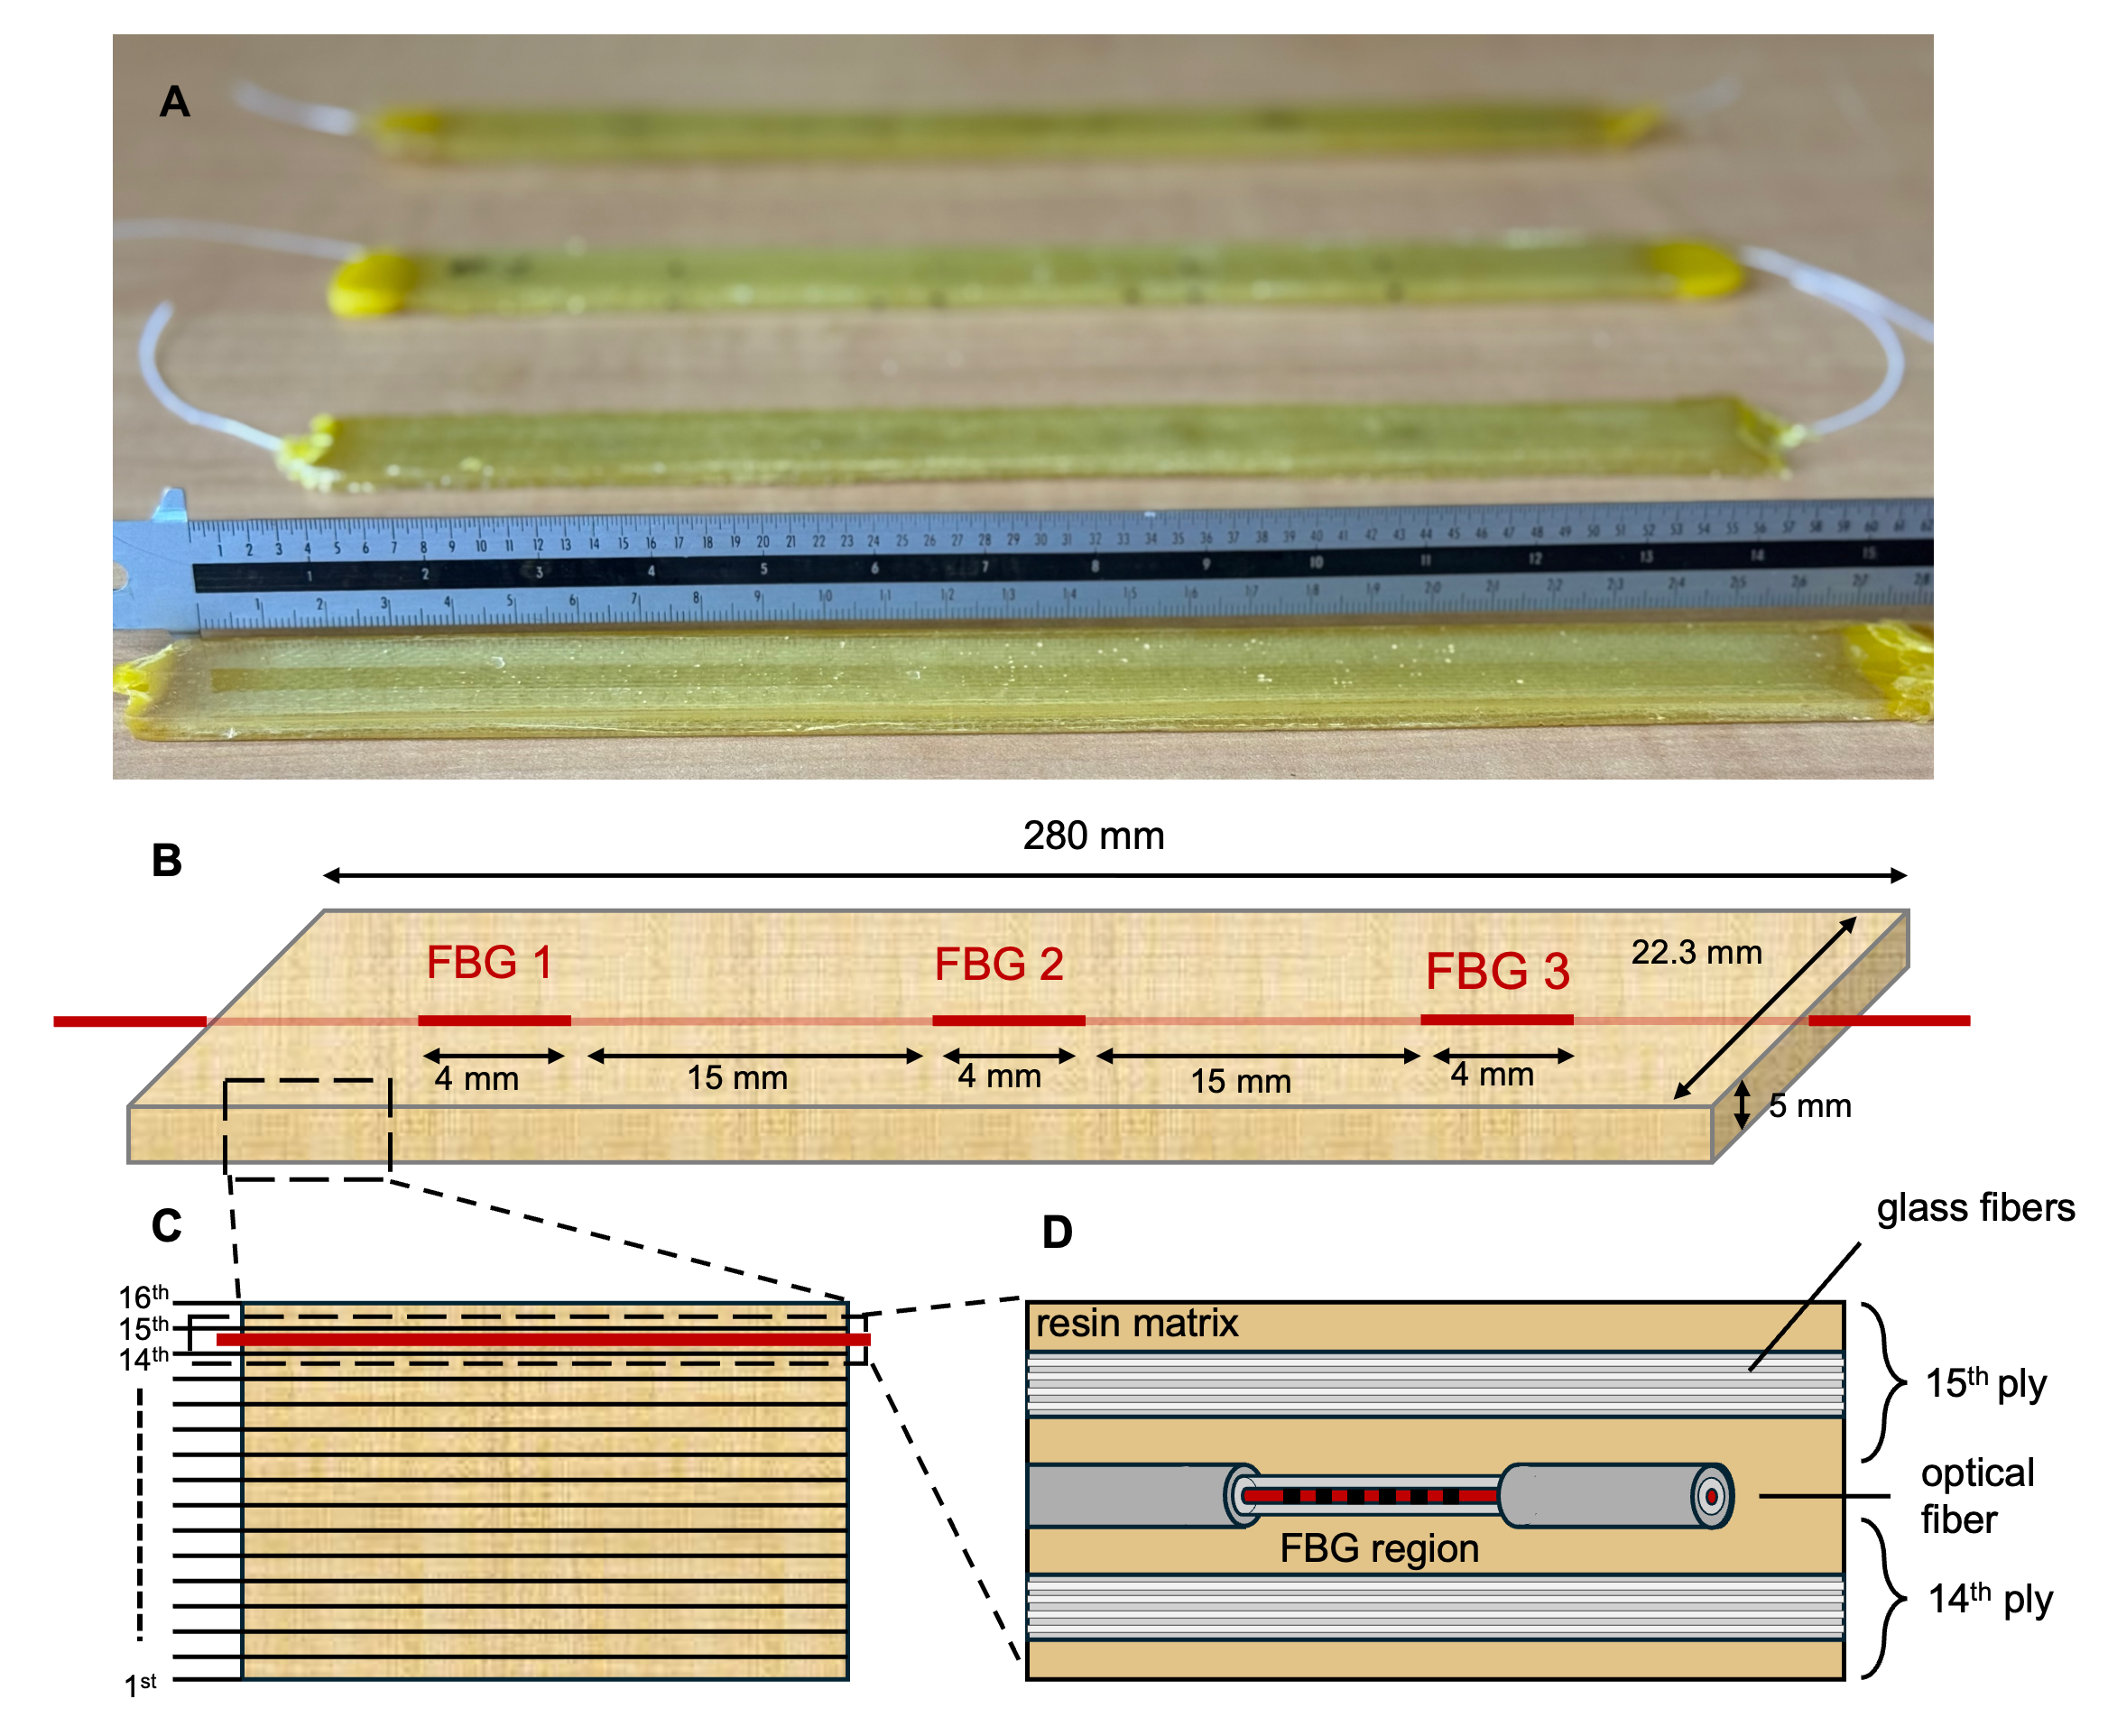
\includegraphics[width=\linewidth]{img/sketch-of-plies-together}
\caption{\textbf{Fabricated composite specimens, specimen geometry, laminate layup, and local sensor embedding.} Panel A shows representative hand laminated glass fiber reinforced polymer specimens used in the three-point bending experiments, with a ruler provided for scale. Panel B shows the specimen geometry, nominal dimensions, and the positions of the three embedded FBGs along the optical fiber. Panel C shows a cross section schematic of the 16-ply laminate, highlighting fiber placement between the 14th and 15th plies near the upper surface. Panel D shows a close view of this interply region, indicating the glass fiber layers, resin matrix, embedded optical fiber, and the FBG sensing region.}
\label{fig:composite_sample}
\end{figure}

\FloatBarrier

\subsection*{Three-point bending experiments}

Mechanical testing was performed with a pneumatic three-point bending system instrumented to measure applied force and crosshead displacement. Each specimen was placed on two supports separated by a prescribed span, and load was applied at midspan. The actuator force was controlled through discrete air pressure settings. For each selected pressure level, ten consecutive loading cycles were applied before moving to the next level. This protocol produced repeated measurements within a given loading block while progressively increasing the loading level on the specimen. During each test, the bending machine recorded force, displacement, and applied pressure, while the embedded FBGs were interrogated in parallel by the BSI-108 FBG interrogator from B-Sens (hereafter referred to as the FBG interrogator). The instrumented bending setup is shown in Figure~\ref{fig:bending_setup}. In the current dataset, support spans of 110, 150, 190, and 230 mm were investigated, and the nominal specimen width was 22.3 mm.

\begin{figure}[htbp]
\centering
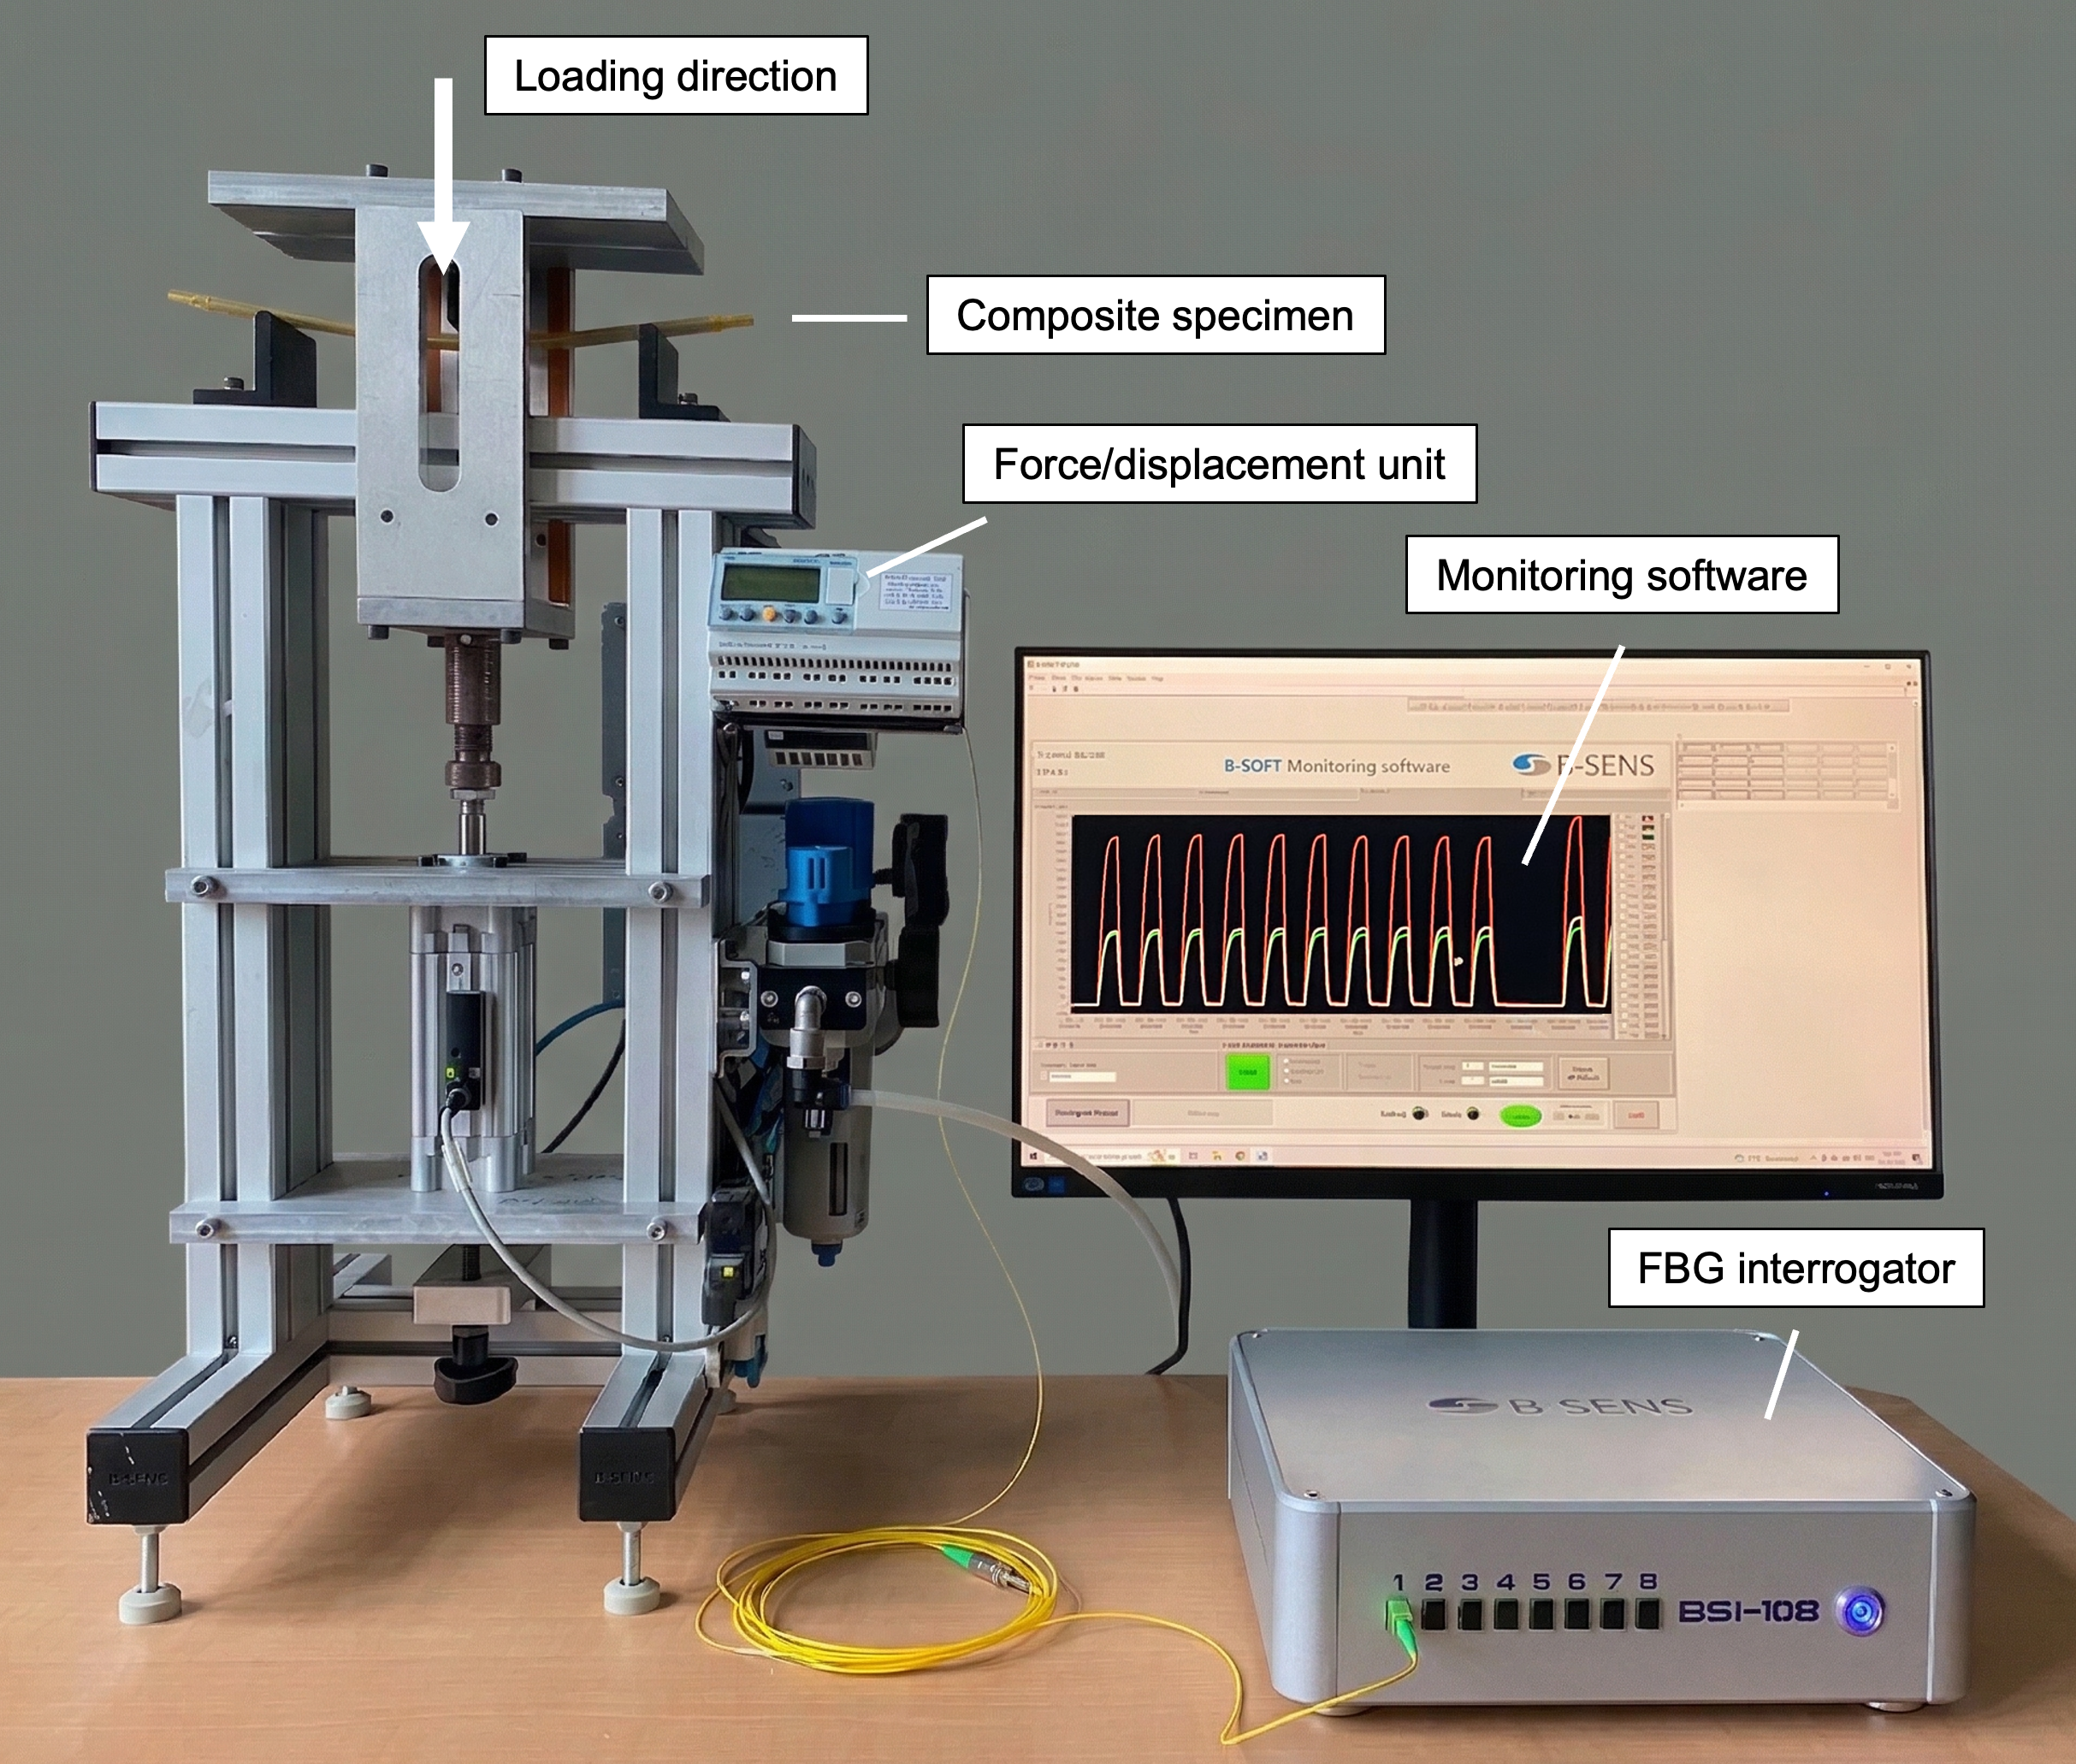
\includegraphics[width=0.7\textwidth, keepaspectratio]{img/experiment-setup-annotated.png}
\caption{\textbf{Three-point bending measurement chain and experimental setup.} Photograph of the instrumented three-point bending system used in the experiments, showing the loading direction, the composite specimen, the force/displacement unit, the monitoring software displayed on the acquisition computer, and the BSI-108 FBG interrogator from B-Sens.}
\label{fig:bending_setup}
\end{figure}

\FloatBarrier

\subsection*{Mechanics based strain interpretation}

The mechanics-informed part of the study is based on the linear elastic response of a slender beam under three-point bending. Similar FBG bending studies have shown that, when embedding is well controlled, the measured wavelength shift can be interpreted consistently with beam theory strain fields in the elastic regime \cite{gabardi2023}. For a simply supported specimen loaded at midspan, the applied force generates a bending moment that produces tension on one side of the beam and compression on the other, while the longitudinal strain vanishes at the neutral axis. An embedded FBG located away from this axis therefore experiences a strain that depends on both the applied load and its position through the thickness. In the present configuration, the maximum bending moment is
\[
M = \frac{F L}{4},
\]
where $F$ is the applied force and $L$ is the support span. According to Euler-Bernoulli beam theory, the longitudinal stress varies linearly with the distance $y$ from the neutral axis \cite{ochsner2021}:
\[
\sigma = \frac{M y}{I},
\]
where $I$ is the second moment of area of the cross section. For the rectangular specimens considered here,
\[
I = \frac{b h^3}{12},
\]
with $b$ the specimen width and $h$ the specimen thickness. Assuming linear elastic behavior before crack initiation, $\varepsilon = \sigma / E$, so the strain at the FBG position becomes
\begin{equation}
\varepsilon = \frac{M y_{\mathrm{FBG}}}{E I} = \frac{3 F L y_{\mathrm{FBG}}}{E b h^3},
\label{eq:euler_bernoulli_strain}
\end{equation}
where $E$ is the effective Young's modulus and $y_{\mathrm{FBG}}$ is the signed distance of the sensor from the neutral axis. This expression provides a simple estimate of the elastic strain expected from an undamaged specimen; deviations between measured and predicted responses therefore motivate the mechanics-informed descriptors used in this work. Before constructing these descriptors, the elastic bending response was examined to verify that beam theory described the behavior before crack initiation. As shown in Figure~\ref{fig:calibration_plots}A, the applied force increased approximately linearly with the measured displacement over the initial loading regime of the calibration specimens. A departure from this linear trend appeared at higher displacement levels, consistent with the onset of nonelastic behavior and supporting the restriction of the mechanics calibration to the regime before crack initiation.

Using the measured wavelength shifts, an FBG strain sensitivity of 1.2 pm/$\mu\varepsilon$ determined from a calibration process, and the Euler-Bernoulli relation in Eq.~\ref{eq:euler_bernoulli_strain}, an effective Young's modulus was estimated from calibration data collected before crack initiation. Figure~\ref{fig:calibration_plots}B shows that the resulting modulus values remained clustered around 18.6 GPa across the investigated force range, with limited dispersion. This supported the use of a single effective modulus of 18.6 GPa for the mechanics-informed analysis, a value consistent with reported elastic moduli for GFRP laminates and woven GFRP composites in the literature \cite{bazli2019,gao2016}. It was then used to compute the elastic strain expected at each loading level and to quantify deviations between measured and expected responses.

\begin{figure}[htbp]
\centering
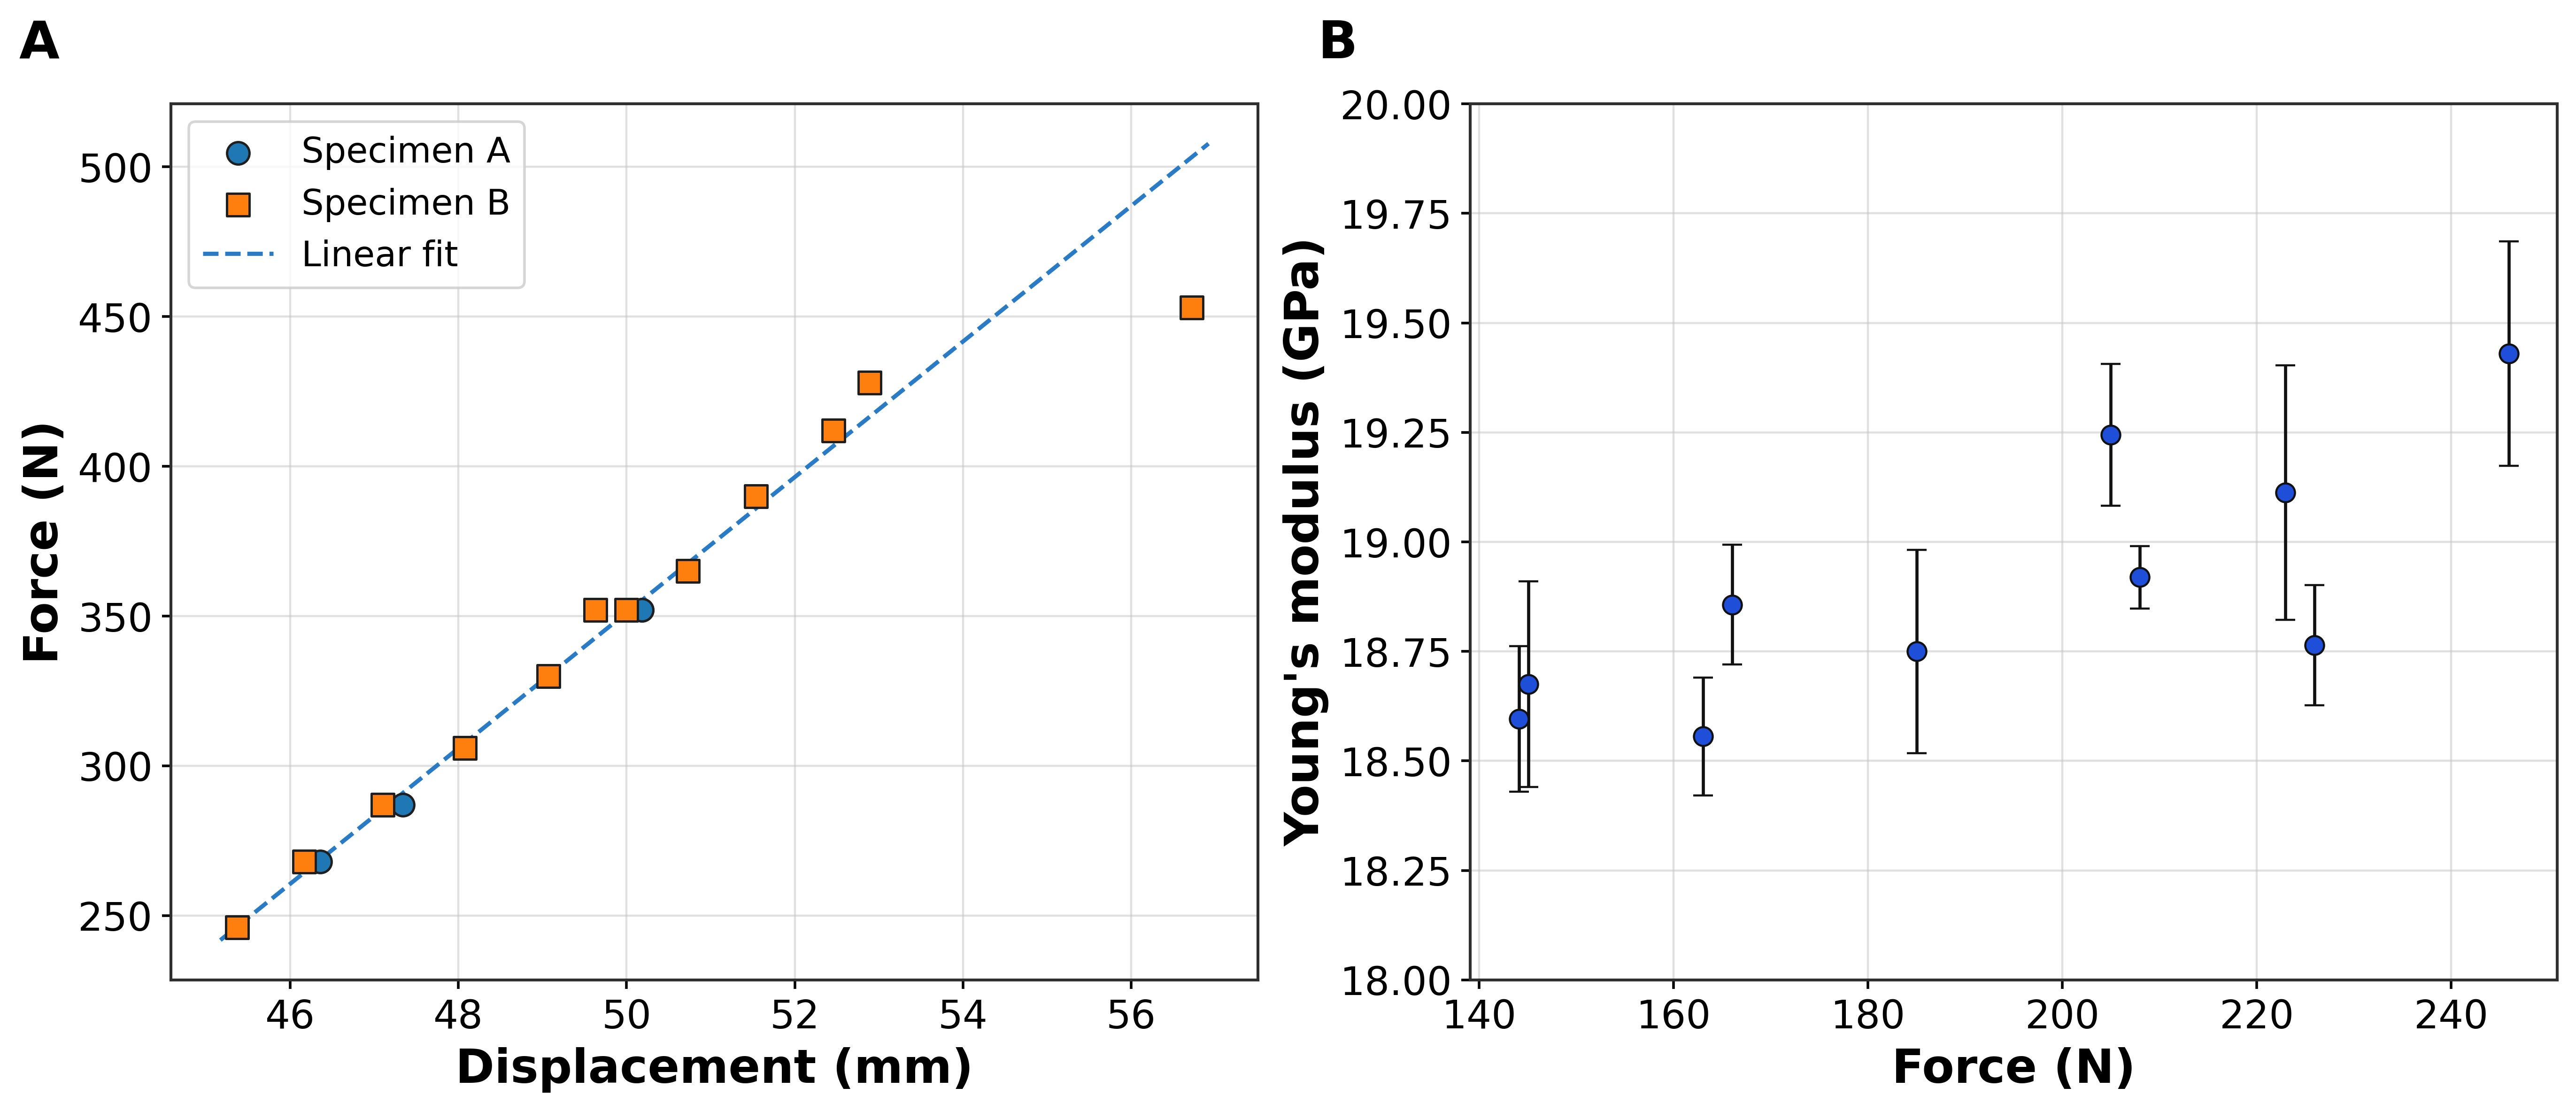
\includegraphics[width=\linewidth]{img/calibration_mechanics_combined}
\caption{\textbf{Calibration of the 16-ply specimens in the elastic regime.} Panel A shows the measured force as a function of displacement for Specimens A and B, together with the fitted linear trend used to identify the initial elastic regime. Panel B shows the effective Young's modulus estimated from calibration measurements before crack initiation using the FBG wavelength shifts and the Euler-Bernoulli bending relation. The limited dispersion across the investigated force range supports the use of a single effective modulus for the mechanics-informed model.}
\label{fig:calibration_plots}
\end{figure}

\FloatBarrier

\subsection*{Data acquisition and interrogator window construction}

The dataset was built from the multiplexed recordings of the FBG interrogator and the synchronized mechanical metadata associated with each experiment. The FBG interrogator tracked the Bragg peak evolution of the active sensor channels at up to 3 kHz over the 1510--1590 nm spectral range, with sub-picometer wavelength resolution. For the present study, each experiment was converted into a sequence of fixed length windows centered on individual loading responses. Each interrogator window contained 50 consecutive samples extracted around a detected peak response and was associated with a window identifier, center time, and crack label. The full dataset comprised 29 experimental runs, each represented by 120 windows centered on peaks and ordered in time, yielding 3,480 labeled windows in total. Because each window retained three synchronized raw channels, this corresponded to 10,440 channel traces of length 50, or 522,000 raw sampled values before constructing the derived signal channels used in the model input.

Mechanical metadata were aligned to the interrogator windows at the level of repeated loading blocks. Each run contained twelve loading groups, and each loading group corresponded to ten consecutive interrogator windows acquired under the same nominal force setting. The force value, support span, specimen thickness, and specimen width were therefore assigned to each window through the combination of experiment identifier and loading group index. For all four controlled variants, each window retained the target interrogator channel together with two companion channels from the same multiplexed acquisition. These three raw channels were later used to construct the signal representation for learning, while the synchronized mechanical metadata were used to derive the optional mechanics descriptors, the auxiliary elastic response target, and the mask identifying windows before crack initiation. Because windows from the same run remained temporally and mechanically correlated, the train, validation, and test partition was kept identical to the reference offline sequence split and applied at the run level so that the controlled comparisons remained matched, meaning that all variants used the same run-wise split, preprocessing pipeline, seed set, and model-selection protocol and differed only in the mechanics descriptors and auxiliary supervision.

Figure~\ref{fig:window_mosaic} shows this hierarchy on one sequence. Panel A shows the full interrogator run together with the loading group selected for closer inspection. Panel B zooms into the corresponding 10-window group and highlights windows before crack initiation and crack windows. Panels C and D then show the individual windows used to illustrate the local waveform changes observed across the multiplexed FBG channels before and after crack initiation.

\begin{figure}[htbp]
\centering
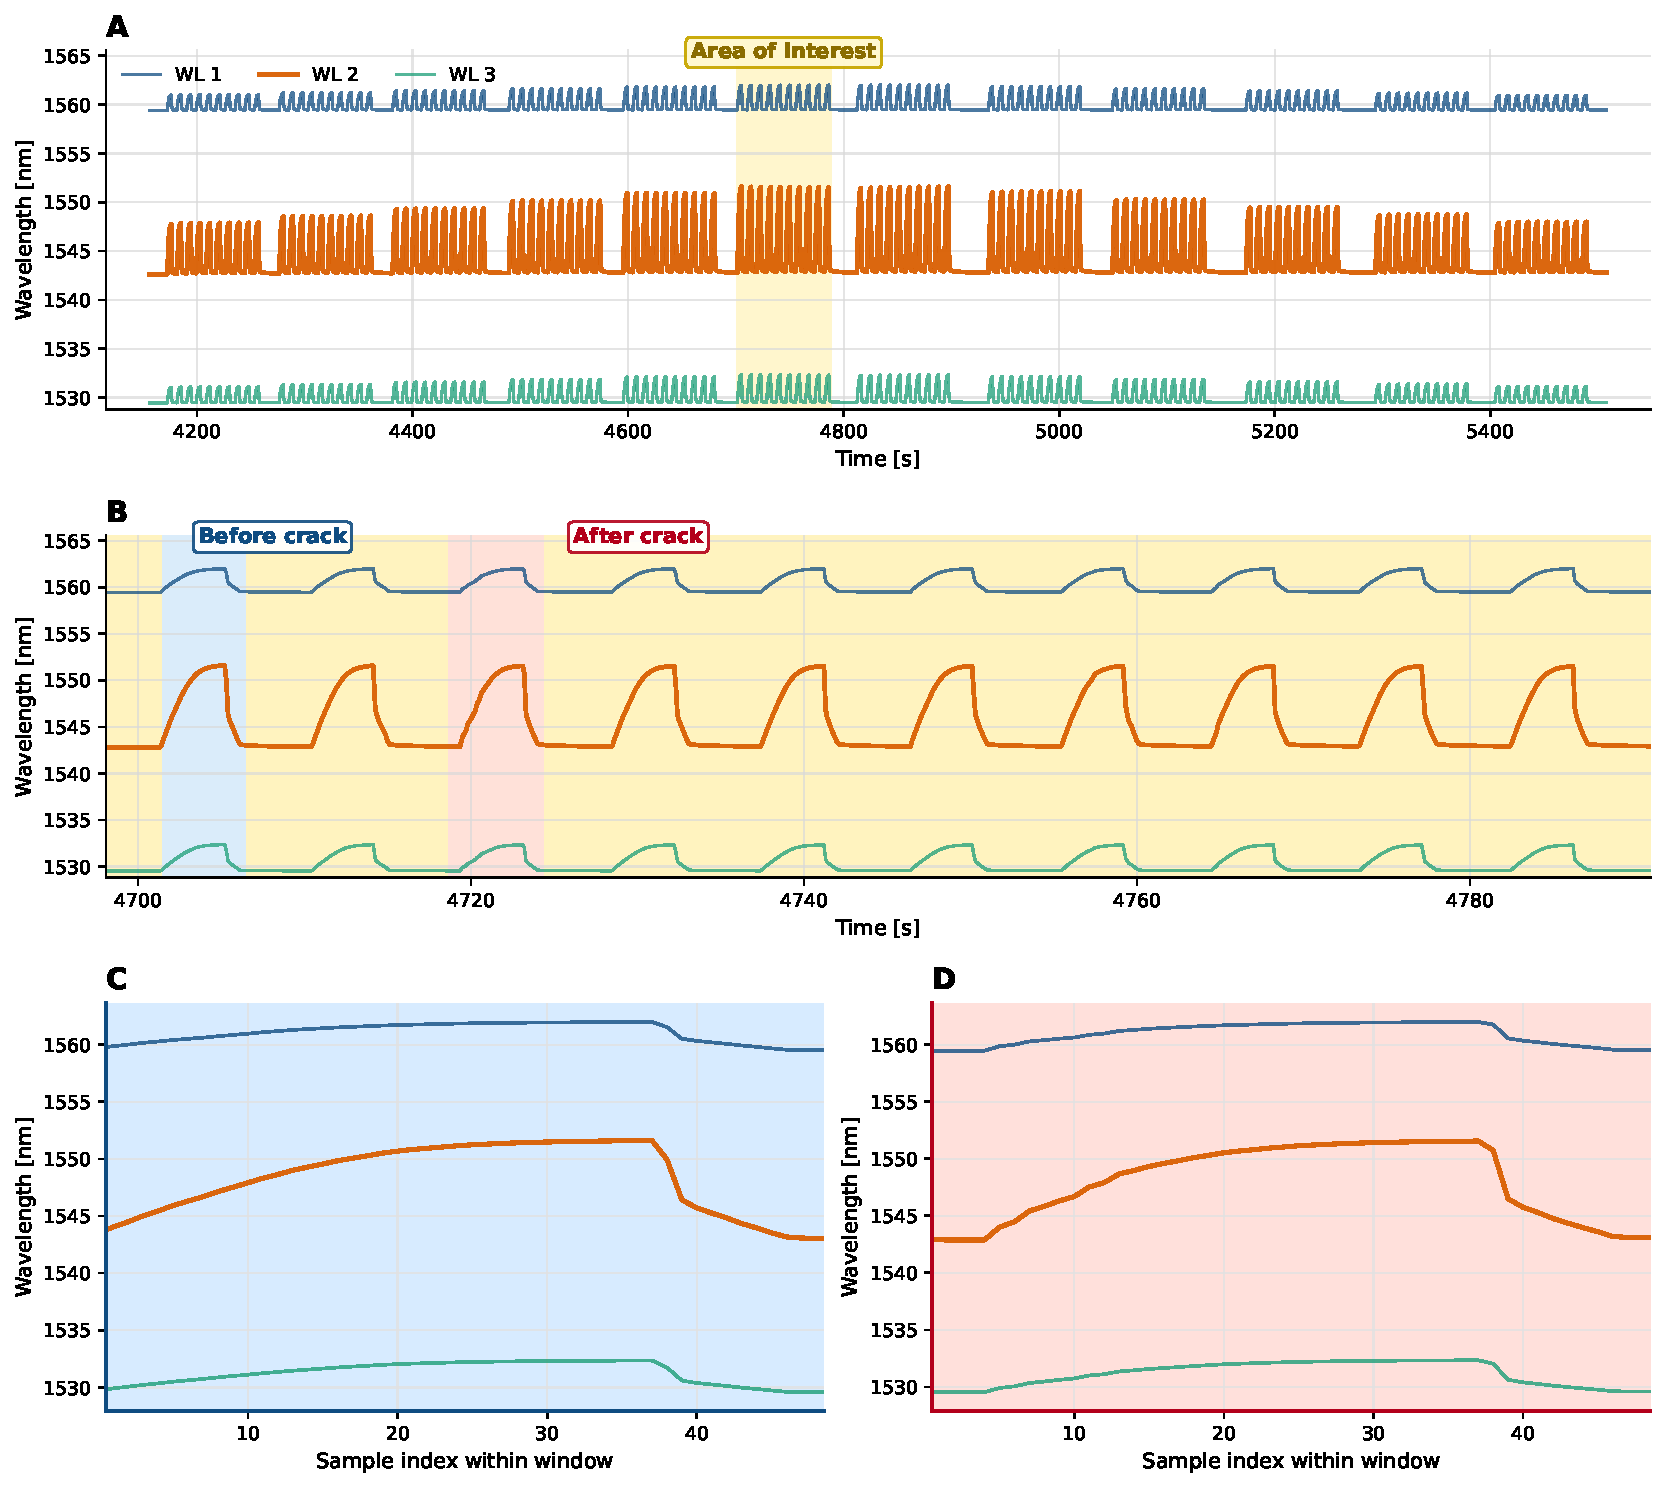
\includegraphics[width=\linewidth]{img/mosaic_time_series_before_after}
\caption{\textbf{Example raw interrogator sequence and window hierarchy used for learning.} Panel A shows the full multiplexed FBG interrogator run, with the selected loading group highlighted. Panel B shows the corresponding 10-window group on a shorter time scale, with windows before crack initiation and crack windows highlighted. Panels C and D show the individual windows before and after crack initiation, respectively, for the target FBG channel together with its two companion channels. This view shows how the raw interrogator signal was organized into loading group context and fixed length windows before feature extraction and learning.}
\label{fig:window_mosaic}
\end{figure}

\FloatBarrier

\subsection*{Input representation and mechanics descriptors}

Each run, that is, one full interrogator measurement sequence from a single specimen test, was represented as a sequence of 120 windows, and each window was represented by a signal tensor together with a scalar descriptor vector. The signal tensor retained the target interrogator channel first, followed by up to two companion channels from the same multiplexed acquisition in file order. For each sensor channel, three aligned derived channels were constructed: the mean centered signal, a first-difference signal computed with edge replication to preserve length 50, and a second-difference signal computed in the same way. The final signal tensor therefore had shape $50\times9$ for every window. This representation keeps the local waveform of the target peak while exposing abrupt changes within each window and responses across channels from the same loading event.

The scalar branch used 15 base descriptors extracted from the target channel. Signal variability was described by the standard deviation, interquartile range, and peak to peak range. Local temporal change was described by the mean absolute first-difference, the standard deviation of the first-difference, the maximum absolute first-difference, and the absolute change in window mean relative to the previous and next windows in the same run. Spectral content was summarized by the mean magnitude in low frequency and high frequency bands of the centered real Fourier spectrum. Cross-channel context was captured by the difference between the target channel mean and the first two companion channel means, together with the ratio of target channel standard deviation to the standard deviation of those companion channels. A final descriptor captured the normalized window position $i/(N-1)$ within the run. Each active base descriptor was also standardized within the same run across its 120 windows, yielding 15 counterparts defined relative to each run and therefore 30 statistical descriptors in total. These descriptors use context from the whole run and are thus part of the offline formulation evaluated here.

Six mechanics descriptors were appended only in variants B and D. The first loading group of each run served as the baseline group. The observed strain change was computed from the difference between the current target channel mean wavelength and the baseline group mean wavelength, converted with the 1.2 pm/$\mu\varepsilon$ FBG sensitivity. The expected elastic strain was computed from Eq.~\ref{eq:euler_bernoulli_strain} using the synchronized force and specimen geometry, a fixed effective modulus of 18.6 GPa, and an FBG distance from the neutral axis set to one third of the specimen thickness. This modulus was fixed before model training from the separate calibration before crack initiation described above and was not re-estimated on the train, validation, or test partitions. The six mechanics descriptors were: applied force, force increment relative to the baseline group, observed strain change, expected strain change relative to the baseline group, the residual between observed and expected strain change, and a normalized residual ratio. The residual ratio divided the residual by $\max(|\Delta\varepsilon_{\mathrm{exp}}|, 50~\mu\varepsilon)$ and was set to zero when the force increment was zero, which avoided unstable values close to the baseline condition. Variants A and C therefore used 30 scalar descriptors, whereas variants B and D used 36. These signal tensor channels and descriptor groups are summarized in Table~\ref{tab:input_summary}.

\begin{table}[htbp]
\centering
\caption{\textbf{Summary of the signal tensor channels and scalar descriptors used by the controlled variants.} All variants used the raw signal tensor. Variants A and C used the 30 statistical descriptors, whereas variants B and D appended the 6 mechanics descriptors for a total of 36 scalar inputs. Final feature standardization was fitted on the training split only.}
\label{tab:input_summary}
\small
\begin{tabular}{p{0.17\linewidth}cp{0.43\linewidth}p{0.24\linewidth}}
\hline
Input group & Count & Exact elements & Notes \\
\hline
Signal tensor channels & 9 channels & Target channel followed by up to two companion channels from the same acquisition, each represented by the mean centered signal, first-difference signal, and second-difference signal computed with edge replication that preserves length & Used in all variants; each window therefore had shape $50\times9$. Runs with only two active channels were zero padded to retain three-channel input \\
Statistical descriptors & 30 & 15 base descriptors: standard deviation, interquartile range, peak to peak range, mean absolute first-difference, standard deviation of the first-difference, maximum absolute first-difference, absolute change in target channel mean relative to the previous and next windows, mean magnitude in low frequency and high frequency bands of the centered real Fourier spectrum, mean gap to companion channels 1 and 2, standard deviation ratio to companion channels 1 and 2, and normalized window position; plus 15 within-run standardized counterparts & Used in variants A--D; descriptors were extracted from the target channel while incorporating temporal and context across channels over the full run \\
Mechanics descriptors & 6 & Applied force, force increment relative to the first loading group, observed strain change from the target wavelength shift, expected elastic strain change from Eq.~\ref{eq:euler_bernoulli_strain}, strain residual, and normalized residual ratio with denominator $\max(|\Delta\varepsilon_{\mathrm{exp}}|, 50~\mu\varepsilon)$ & Appended only in variants B and D; the effective modulus was fixed at 18.6 GPa before model training \\
\hline
\end{tabular}
\end{table}

\FloatBarrier

After all signal tensor channels and scalar descriptors had been constructed, the nine signal channels were standardized using channel means and standard deviations estimated only from the training split and aggregated over runs, windows, and within window samples. The scalar descriptors were standardized in the same way using training split statistics aggregated over runs and windows. Dataset construction rejected windows with invalid indices or missing channel values; the 29 retained runs passed this check and were written to the archived train, validation, and test files without imputation.

\subsection*{Mechanics-informed multiscale temporal CNN}

The proposed model is summarized in Figure~\ref{fig:physics_architecture}. It combines a multiscale signal feature extractor, a scalar-descriptor branch, and a run-level temporal convolutional module. During training, each batch contained 4 runs, where each run denotes one full interrogator measurement sequence represented by 120 ordered windows. The signal input therefore had shape $4\times120\times50\times9$ and the descriptor input had shape $4\times120\times30$ for variants A and C or $4\times120\times36$ for variants B and D. The model first processes each window independently and then models the ordered sequence of 120 windows within a run.

The signal branch processed each nine-channel, 50-sample window using three parallel one-dimensional convolutional branches with kernel sizes 3, 7, and 15. A multiscale one-dimensional CNN was used because the relevant crack signatures in this problem appear as short local waveform changes within a window rather than as spatial patterns, and their characteristic width was not known a priori. The three branches therefore allowed the model to examine each window at fine, intermediate, and broader scales within the same 50-sample segment. In each branch, a convolution from 9 to 32 channels was followed by a Gaussian Error Linear Unit (GELU) and batch normalization, and then by a second convolution from 32 to 48 channels, GELU, batch normalization, adaptive average pooling to length 1, and flattening. GELU was used to preserve small waveform differences without a hard cutoff. In the implemented architecture, the second convolution used kernel sizes 3, 3, and 7 for the branches that started with 3, 7, and 15, respectively. This produced two-layer receptive fields of 5, 9, and 21 samples, which let the branch summarize local peak morphology over short, intermediate, and broader spans within the 50-sample window. The three 48-dimensional outputs were concatenated into a 144-dimensional vector and projected by a fully connected (linear) layer, GELU, and layer normalization to a 160-dimensional signal representation.

The descriptor branch applied layer normalization to a 30- or 36-element scalar vector, followed by a 64-unit fully connected layer, GELU, dropout, a 32-unit fully connected layer, GELU, and a final layer normalization. The descriptor branch was kept separate so that engineered summaries and raw temporal waveforms were processed separately before fusion. The resulting descriptor representation of size 32 was concatenated with the signal representation of size 160. A fusion block then mapped the combined 192-dimensional vector back to 160 dimensions through a fully connected layer, GELU, layer normalization, and dropout.

Run level context was modeled with six residual temporal convolution blocks using kernel size 3, dropout 0.25, and dilation factors 1, 2, 4, 8, 16, and 32. Residual dilated temporal convolutions were used because crack related behavior can extend over several neighboring windows, and dilation enlarges the temporal field of view across the run of 120 windows without reducing window resolution. Each block contained two same-width convolutions from 160 to 160 channels, each followed by batch normalization and GELU, and the residual connection was added before the final activation. A classification head composed of layer normalization, a 64-unit fully connected layer, GELU, dropout, and a final fully connected output layer produced one logit per window. In parallel, a direct linear shortcut from the active scalar descriptor vector to the output logit allowed engineered descriptors to contribute without passing only through the temporal stack. This shortcut let informative mechanics and context descriptors affect the crack score directly rather than only after temporal mixing. The configuration with 36 features contains approximately 1.06 million trainable parameters (1,061,727 parameters for the model with 36 features).

An auxiliary mechanics head was attached to the 160-dimensional signal representation before feature fusion. This head consisted of layer normalization, a 64-unit fully connected layer, GELU, dropout, and a final fully connected output layer predicting the expected elastic strain change for each window. Its loss was evaluated only on healthy windows and only in variants C and D. Restricting this loss to healthy windows avoids forcing responses after crack initiation to match an elastic target. This architecture separates three types of information present in the archived benchmark: local waveform morphology inside each 50 sample interrogator window, scalar descriptors summarizing behavior within and across windows, and longer range temporal structure across the run of 120 windows.

\begin{figure}[htbp]
\centering
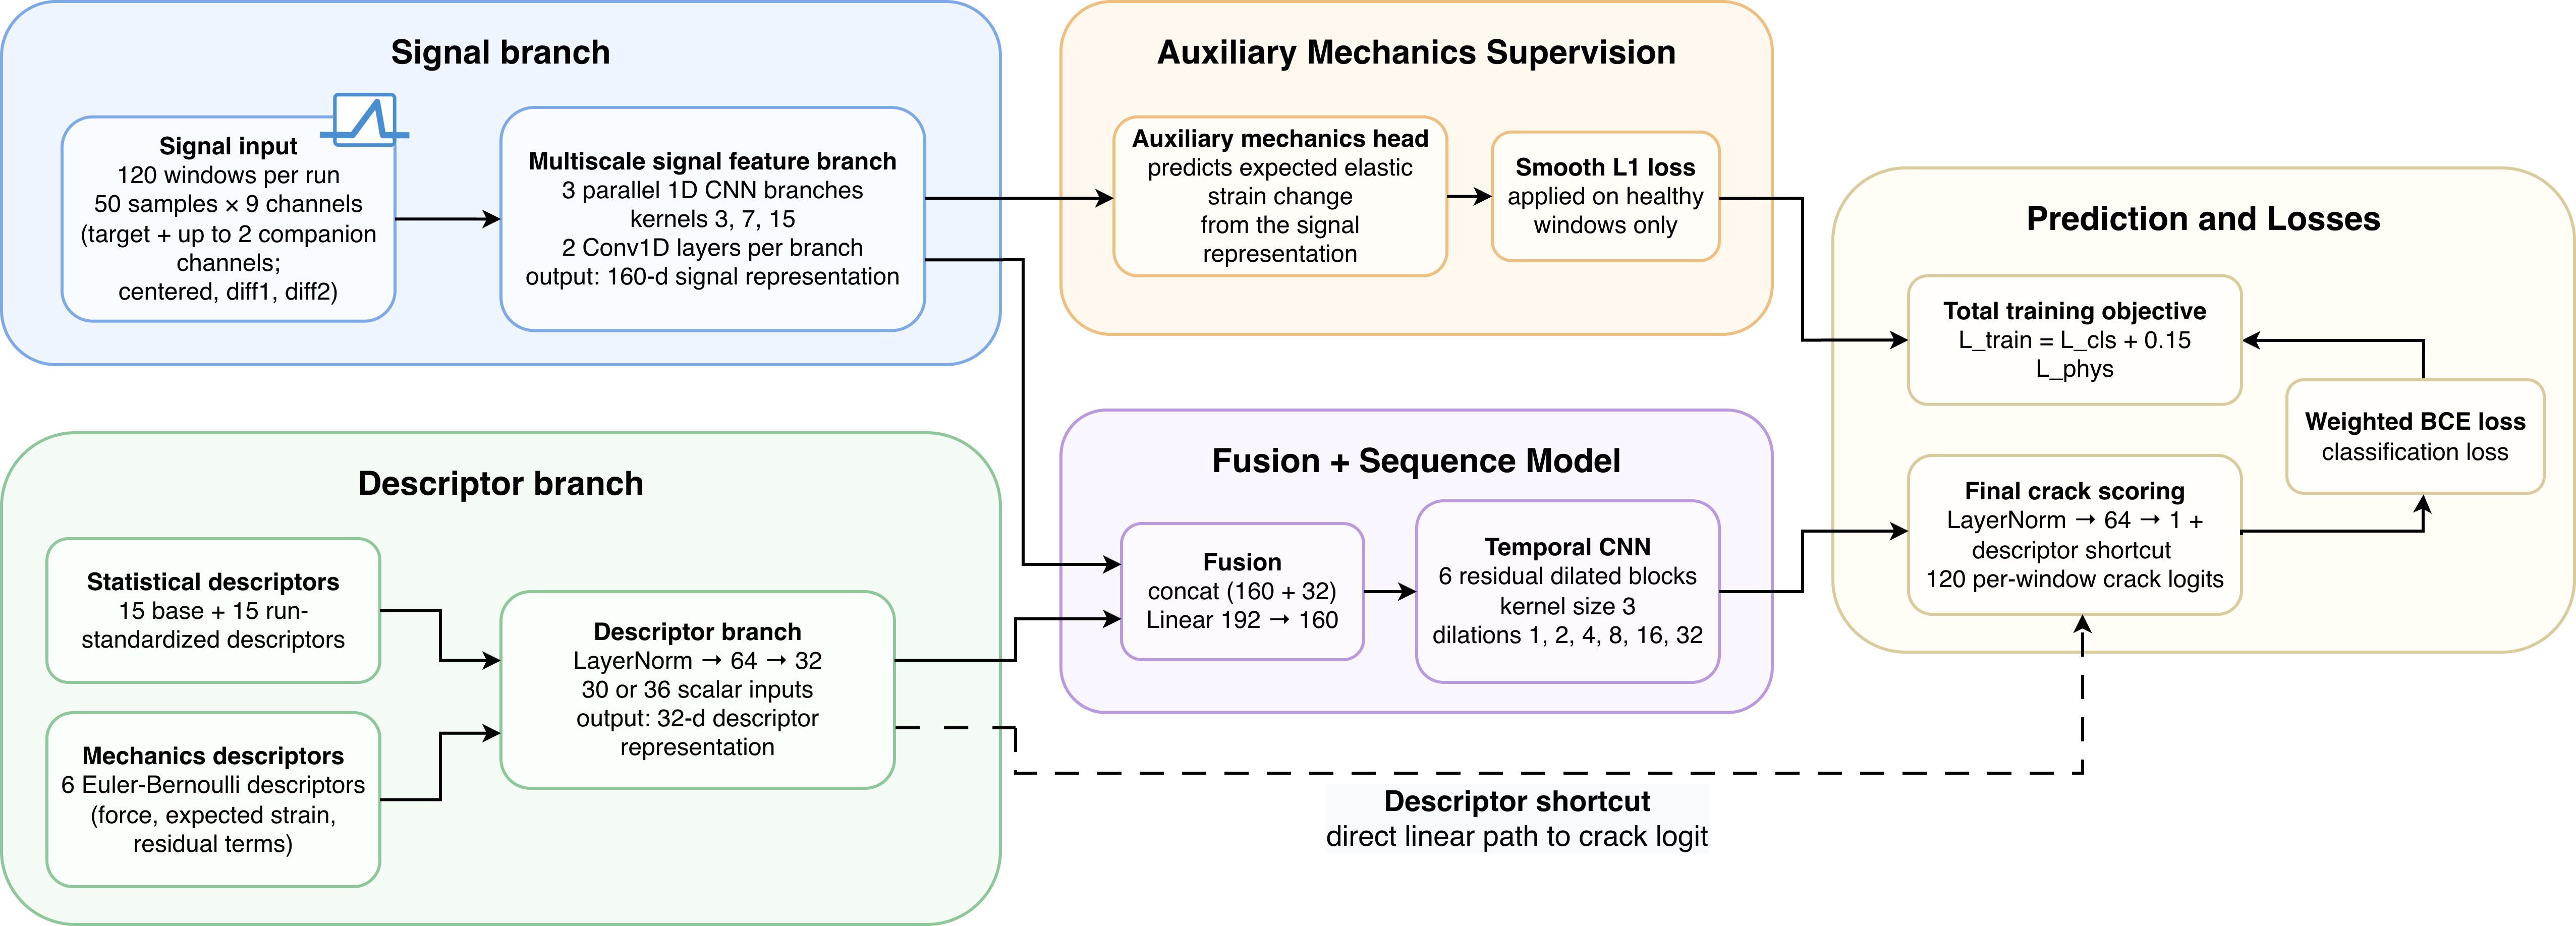
\includegraphics[width=\linewidth]{img/neural-network.drawio.updated.png}
\caption{\textbf{Mechanics-informed multiscale temporal CNN used for crack localization.} Each interrogator window is represented by a $50\times9$ signal tensor obtained from the target channel and up to two simultaneously acquired companion channels, together with a descriptor vector comprising 30 statistical descriptors and, when enabled, an appended set of 6 Euler--Bernoulli mechanics descriptors. The signal tensor is processed by a three-branch one-dimensional convolutional feature extractor with kernel sizes 3, 7, and 15, the active descriptor vector is processed by a small multilayer perceptron, and both learned representations are fused before temporal convolution across the 120-window run sequence. A classification head produces one crack logit per window, with an additional direct descriptor shortcut to that logit. Crack localization is supervised by a weighted binary cross-entropy loss, while an auxiliary mechanics head predicts the expected healthy elastic strain change and contributes a Smooth L1 loss on healthy windows only when auxiliary supervision is enabled.}
\label{fig:physics_architecture}
\end{figure}

\FloatBarrier

\subsection*{Training, model selection, and evaluation}

All four controlled variants were trained on the same train/validation/test run split so that the effects of descriptor augmentation and auxiliary supervision could be assessed without changing the evaluation protocol. Training combined a weighted binary cross entropy loss for crack localization with an auxiliary Smooth L1 loss (SmoothL1Loss in PyTorch) for elastic strain prediction on healthy windows only, that is, a robust regression loss that is quadratic for small errors and linear for larger ones:
\begin{equation}
\mathcal{L} = \mathcal{L}_{\mathrm{cls}} + \lambda \mathcal{L}_{\mathrm{phys}},
\end{equation}
where $\lambda = 0$ for variants A and B and $\lambda = 0.15$ for variants C and D. The classification loss was applied to all 120 windows in each run and used a positive class weight computed from the training split to address class imbalance. For the archived split, this weight was $1535/385 = 3.99$. The auxiliary Smooth L1 term was computed element wise on the predicted elastic strain change, multiplied by the healthy mask, and normalized by the number of healthy windows in the batch. The auxiliary loss was therefore inactive for variants A and B and active only on windows before crack initiation for variants C and D.

Model optimization used AdamW with a learning rate of $4\times10^{-4}$ and weight decay of $2\times10^{-4}$. Training was performed for up to 80 epochs with a batch size of 4 runs. To reduce sensitivity to small perturbations in the interrogator traces, additive Gaussian noise with a standard deviation of 0.01 was applied to the signal tensor only during training. Gradients were clipped to a norm of 1.0. The learning rate was scheduled with PyTorch's ReduceLROnPlateau using the validation loss as the monitored quantity. If the validation loss did not improve for 5 consecutive epochs, the optimizer learning rate was reduced by a factor of 0.5, down to a minimum of $10^{-5}$. This scheduler only adjusted the optimization step size and did not terminate training. Four random initializations (seeds 7, 11, 23, and 42) were evaluated, and early stopping was applied separately, terminating training only after 14 consecutive epochs without improvement in the validation selection criterion.

At the end of each epoch, the validation probabilities were converted into binary predictions by selecting a validation thresholding rule. Two thresholding families were considered. The first was a global threshold scanned from 0.05 to 0.90 in steps of 0.01. The second was a threshold defined for each run, of the form $\max(\mathrm{floor}, \mu + s\sigma + b)$, where $\mu$ and $\sigma$ are the mean and standard deviation of the predicted probabilities within a validation run, $b\in\{-0.25,-0.125,0,0.025\}$, $s\in\{0.3,0.4,0.6,1.3\}$, and $\mathrm{floor}\in\{0.1,0.15,0.2,0.25,0.3,0.35\}$. Probability smoothing was available in the post-processing code but was fixed to a window size of 1, that is, no additional smoothing, for all results reported here.

Checkpoint selection and early stopping were based on validation metrics after application of the selected thresholding rule rather than on raw validation loss alone. Because missed crack windows were treated as more costly than false alarms, model selection prioritized validation $F_2$, then recall, and finally balanced accuracy. The $F_2$ score was preferred because it weights recall more heavily than precision, which is appropriate for a warning task in which missed crack windows are more problematic than extra alerts. Balanced accuracy was used only as a final tie-break when $F_2$ and recall were effectively tied. Each seed therefore produced one checkpoint selected on validation and one associated thresholding rule, which were applied unchanged to the held out test runs. The training script also evaluated simple probability averaging ensembles across seeds as a validation reference, but the reported manuscript tables use only results from individual models. All reported metrics are pooled metrics at window level on the flattened test windows after application of the validation-selected thresholding rule, except the receiver operating characteristic area under the curve (ROC-AUC), which was computed from the raw window probabilities before thresholding. ROC-AUC measures how well the model ranks crack windows above windows without cracks across all possible thresholds, so it complements the threshold dependent metrics reported after threshold selection. Unless stated otherwise, Table~\ref{tab:overall_performance} reports mean $\pm$ standard deviation across the four test results from individual seeds, whereas Table~\ref{tab:ablation_summary} reports a validation-selected single-model supporting analysis rather than averages over seeds.

\section*{Results}

\subsection*{Offline crack localization performance}

The offline evaluation used the same 5 test runs (600 windows in total), the same split by run, and the same validation-selected thresholding protocol described in Methodology. Table~\ref{tab:overall_performance} provides the primary matched comparison and reports mean $\pm$ standard deviation across the same four seeds. This comparison isolates the contributions of descriptor augmentation and auxiliary supervision without changing the evaluation protocol. The full mechanics-informed variant D yielded the best mean performance across seeds, with precision $= 0.773 \pm 0.053$, $F_1 = 0.819 \pm 0.029$, $F_2 = 0.850 \pm 0.020$, balanced accuracy $= 0.897 \pm 0.015$, and ROC-AUC $= 0.968 \pm 0.012$. Variant B reached the highest mean recall ($0.880 \pm 0.039$), while variant D remained close in recall ($0.873 \pm 0.024$) and gave the best balance across the reported metrics. Separate validation-selected single-model results from supporting analyses were retained for interpretive reference, whereas the main manuscript comparison reports mean $\pm$ standard deviation across four seeds.

\begin{table}[htbp]
\centering
\caption{\textbf{Primary four-seed matched comparison of mechanics descriptors and auxiliary loss.} All four variants used the same split by run, preprocessing, temporal backbone, seed set, model selection rule, and validation threshold search. Values are pooled metrics at window level on the 600 test windows and are reported as mean $\pm$ standard deviation across four validation-selected models, one per seed. Variant A is the matched baseline, variant B adds mechanics descriptors only, variant C adds auxiliary loss only, and variant D combines both. Abbreviations in the table: Var., variant; desc., descriptors; Bal., balanced.}
\label{tab:overall_performance}
\small
\begin{tabular}{llcccccc}
\hline
Var. & Label & Precision & Recall & $F_1$ & $F_2$ & Bal. accuracy & ROC-AUC \\
\hline
A & matched baseline & 0.743 $\pm$ 0.032 & 0.816 $\pm$ 0.069 & 0.776 $\pm$ 0.031 & 0.799 $\pm$ 0.051 & 0.865 $\pm$ 0.029 & 0.959 $\pm$ 0.005 \\
B & mechanics desc. & 0.725 $\pm$ 0.033 & 0.880 $\pm$ 0.039 & 0.795 $\pm$ 0.022 & 0.844 $\pm$ 0.028 & 0.889 $\pm$ 0.018 & 0.961 $\pm$ 0.009 \\
C & auxiliary loss & 0.749 $\pm$ 0.031 & 0.859 $\pm$ 0.069 & 0.798 $\pm$ 0.019 & 0.833 $\pm$ 0.047 & 0.885 $\pm$ 0.025 & 0.966 $\pm$ 0.004 \\
D & both additions & 0.773 $\pm$ 0.053 & 0.873 $\pm$ 0.024 & 0.819 $\pm$ 0.029 & 0.850 $\pm$ 0.020 & 0.897 $\pm$ 0.015 & 0.968 $\pm$ 0.012 \\
\hline
\end{tabular}
\end{table}

\FloatBarrier

\subsection*{Effect of mechanics-informed learning}

To quantify the mechanics-informed formulation without combining multiple changes, four matched variants were evaluated under the same split, seeds, preprocessing, model selection rule, and validation threshold search. Variant A is the matched baseline model using raw signals and 30 statistical descriptors only. Variant B adds the six mechanics descriptors while keeping auxiliary supervision off. Variant C is the auxiliary loss only condition: the classifier still receives only raw signals and statistical descriptors, but the signal branch is additionally trained with the auxiliary target based on mechanics on healthy windows. Variant D combines both the six mechanics descriptors and the auxiliary loss term.

This design enables four pairwise comparisons from Table~\ref{tab:overall_performance}. The contrast A versus B isolates the effect of the mechanics descriptors. Relative to the matched baseline, variant B increased mean recall from $0.816 \pm 0.069$ to $0.880 \pm 0.039$ and mean $F_2$ from $0.799 \pm 0.051$ to $0.844 \pm 0.028$, with a small decrease in precision from $0.743 \pm 0.032$ to $0.725 \pm 0.033$. The contrast A versus C isolates the effect of auxiliary supervision without the six mechanics descriptors in the classifier input. Variant C improved mean $F_1$ from $0.776 \pm 0.031$ to $0.798 \pm 0.019$, balanced accuracy from $0.865 \pm 0.029$ to $0.885 \pm 0.025$, and ROC-AUC from $0.959 \pm 0.005$ to $0.966 \pm 0.004$, while also increasing recall to $0.859 \pm 0.069$.

The contrast B versus D measures the effect of auxiliary supervision once the mechanics descriptors are already present. Relative to variant B, variant D mainly improved precision ($0.773 \pm 0.053$ vs. $0.725 \pm 0.033$), $F_1$ ($0.819 \pm 0.029$ vs. $0.795 \pm 0.022$), and ROC-AUC ($0.968 \pm 0.012$ vs. $0.961 \pm 0.009$), with only a slight decrease in recall ($0.873 \pm 0.024$ vs. $0.880 \pm 0.039$). Compared with the matched baseline, the full mechanics-informed variant improved all reported mean metrics, including $F_1$ by 0.043, $F_2$ by 0.051, balanced accuracy by 0.032, and ROC-AUC by 0.009, indicating that both mechanics descriptors and auxiliary supervision contribute to the improvement. Table~\ref{tab:overall_performance} provides the primary evidence because it reports mean $\pm$ standard deviation across the same four seeds, whereas Table~\ref{tab:ablation_summary} reports a validation-selected single-model supporting analysis and should not be compared numerically row by row against Table~\ref{tab:overall_performance}. A supporting sensitivity check of the auxiliary loss weight within the descriptor-enabled setting showed broadly stable performance across the tested values of $\lambda$, with no consistent improvement across all metrics; $\lambda = 0.15$ was therefore retained for the main controlled comparison.

\subsection*{Interpreting the learned input representation}

Because variant A retains the raw signal representation and handcrafted statistical descriptors without mechanics augmentation, Table~\ref{tab:ablation_summary} provides supporting information for interpreting which non-mechanics inputs affect localization performance. These values come from individual models selected on validation and should therefore be read as supporting single-model ablations, not as averages over multiple seeds. The reference row comes from the validation-selected single-model baseline summary, the descriptor group rows come from the seed 11 feature ablation sweep on the non-mechanics baseline configuration, and the signal-channel ablation rows come from the corresponding signal ablation summaries for the same baseline configuration. Removing the temporal change descriptor family caused the largest degradation, reducing $F_1$ from 0.811 to 0.761 and ROC-AUC from 0.960 to 0.939. This indicates that abrupt local changes within and between windows have the largest effect on localization performance.

Removing the cross-channel descriptor family caused the largest loss in sensitivity, reducing recall from 0.921 to 0.764 and $F_2$ from 0.874 to 0.778. At the raw signal level, using only the target channel preserved $F_1$ almost exactly (0.811 vs. 0.811) but reduced recall to 0.814 and $F_2$ to 0.813. Together, these results show that companion interrogator channels mainly affect recall more than precision. Removing the first-difference channel led to a smaller decline ($F_1 = 0.803$, recall $= 0.843$), consistent with recent FBG studies in which array dynamics, multispectral fusion, and sensor fusion features improve damage sensitivity \cite{wang2023,zhao2025,xiong2025}.

\begin{table}[htbp]
\centering
\caption{\textbf{Supporting validation-selected single-model ablations for the non-mechanics baseline representation.} This table reports pooled ablations at window level on the baseline configuration without mechanics, using individual models selected on validation. These values are not seed-averaged and are not directly numerically comparable to Table~\ref{tab:overall_performance}. The reference row corresponds to the validation-selected single-model baseline summary, descriptor family rows correspond to the seed 11 feature ablation sweep, and signal-channel ablation rows correspond to the corresponding signal ablation summaries. Descriptor ablations isolate the contribution of the handcrafted statistical feature groups, whereas signal ablations probe the role of companion channel information and first-difference information in the raw signal representation.}
\label{tab:ablation_summary}
\small
\begin{tabular}{p{0.48\linewidth}cccc}
\hline
Single-model supporting analysis & Recall & $F_1$ & $F_2$ & ROC-AUC \\
\hline
Single-model baseline & 0.921 & 0.811 & 0.874 & 0.960 \\
Descriptor ablation: drop temporal change & 0.843 & 0.761 & 0.808 & 0.939 \\
Descriptor ablation: drop cross-channel descriptors & 0.764 & 0.799 & 0.778 & 0.966 \\
Signal ablation: target channel only & 0.814 & 0.811 & 0.813 & 0.967 \\
Signal ablation: drop first-difference channel & 0.843 & 0.803 & 0.826 & 0.967 \\
\hline
\end{tabular}
\end{table}

\FloatBarrier

\section*{Discussion}

These results indicate that crack localization is feasible directly from short raw windows of multiplexed FBG interrogator data. In the matched four variant comparison, adding mechanics information improved the baseline, and the full variant D gave the best overall balance across precision, $F_1$, $F_2$, balanced accuracy, and ROC-AUC while keeping recall close to the highest value observed in variant B. This matters because the method operates on short raw interrogator windows rather than dense distributed sensing fields or reduced spectral indicators. The results therefore support the view that the raw multiplexed signals contain localized damage information when the model is given enough temporal context, companion channel context, and mechanics context.

The main interpretation should come from Table~\ref{tab:overall_performance}, the controlled A/B/C/D comparison, because it isolates descriptor augmentation and auxiliary supervision under the same split, preprocessing, architecture, seeds, model selection rule, and validation threshold search. The supporting single-model analysis in Table~\ref{tab:ablation_summary} is useful for interpretation only and should not be compared numerically row by row against Table~\ref{tab:overall_performance}. In that matched setting, variant B mainly increased recall relative to variant A, which suggests that the mechanics descriptors helped the model recover more crack windows. Variant C improved $F_1$, balanced accuracy, and ROC-AUC relative to variant A, which suggests that the auxiliary mechanics target improved representation learning even when the classifier input did not include the six mechanics descriptors. Variant D then improved precision, $F_1$, and ROC-AUC relative to variant B while keeping recall close, which suggests that descriptor augmentation and auxiliary supervision contributed in different ways and were complementary.

One reason for this pattern may be that the mechanics terms capture departures from an expected elastic response rather than only raw waveform variation. The appended descriptors summarize force level, strain change, and residual mismatch with the Euler-Bernoulli estimate, so they provide a compact description of how each window differs from an elastic baseline before damage. The auxiliary head adds a related training constraint by asking the signal representation to predict the expected elastic strain change on healthy windows only. Crack initiation is expected to appear as a deviation from the elastic response seen before damage, so this supervision may help organize pre-crack signal variation in a way that makes later departures easier to separate. This does not mean that the network learns mechanics in a strict sense. Rather, the results suggest that descriptors based on mechanics and a pre-crack elastic target provide structure that is useful for localization.

The supporting descriptor and signal ablations help clarify what the baseline without mechanics already captures. Among the descriptor groups, removing the temporal change descriptors caused the largest drop in $F_1$ and ROC-AUC, which suggests that local change across and within windows is an important part of the crack signature in this dataset. Cross-channel descriptors had their largest effect on recall, and the target channel only signal representation preserved $F_1$ but reduced recall and $F_2$. Taken together, these patterns suggest that companion channels mainly improve sensitivity by helping the model recover more crack windows rather than by simply improving precision. Removing the first-difference channel produced a smaller decline, so derivative-like signal channels still help, but their role appears smaller than that of the temporal change descriptor family. Because these ablations come from validation-selected individual models rather than from the controlled comparison averaged across seeds, they should be treated as supporting interpretive evidence rather than as a definitive ranking of input importance.

In conclusion, these findings differ from much of the prior literature in two ways. Prior FBG learning studies have often relied on engineered features, fused representations, or specimen level labels rather than direct localization from short raw interrogator windows \cite{chilelli2019,zhang2020,wang2023,zhao2025,xiong2025,saha2025}. By contrast, distributed fiber optic studies often operate on richer spatial fields that make localization more direct but depend on denser measurements \cite{liu2023,lu2025}. The present study extends prior FBG learning work by targeting crack localization at the window level from short raw multiplexed signals while adding mechanics structure from synchronized load and geometry metadata. This is also consistent with broader SHM work showing that learned models can benefit from structural priors when sensing data alone are limited \cite{yoon2022,moreh2025,si2025}.

\section*{Data availability}

All data are available upon reasonable request to the corresponding author.

\section*{Code availability}

The code used in this study is available from the corresponding author upon reasonable request.

\bibliography{sample}

\section*{Funding}

The authors acknowledge financial support from Walloon Region of Belgium through the Interreg VI France-Wallonie-Vlaanderen program co-funded by the European Union, under SALOME project (No. 0100240). This work was also supported by WEL Research Institute and the Fonds de la Recherche Scientifique (F.R.S.--FNRS).

\section*{Acknowledgments}

The authors thank Mariel David for her assistance during the manufacturing of the composite specimens. The authors also thank Damien Kinet from B-SENS for his assistance with the operation of the three-point bending system.


\section*{Author contributions statement}

A.U. analyzed the data, applied the machine learning algorithm, and contributed to writing the manuscript. A.G. supervised the machine learning aspects of the study. E.N. and T.T. cured the composite specimens and conducted the three-point bending experiments. K.Y. supervised the FBG-related aspects of the study. K.C. assisted with FBG inscription and curing of the composite specimens. C.C. supervised the FBG-related aspects of the study and wrote the manuscript.

\section*{Additional information}

Competing interests: The authors declare no competing interests.

\end{document}
